\chapter{Programming process}
\label{progprocess}
In this chapter, the programming language and usage of packages would be introduced briefly. Then, some assumptions would be stated, which have a strong influence on modelling and processing. The programming process would be elaborated in final.
\section{Python}
In this project, Python, which is an interpreted high-level general-purpose programming language, is used to analyze data and find the optimum path.
\\The benefits of choosing Python for this project are:
\begin{enumerate}[a)]
    \item Python is versatile, readable, well-structured and easy to use and read
    \item Extensive support libraries make it easy to plot and handle data
\end{enumerate}
However, disadvantages are linked with these benefits:
\begin{enumerate}[a)]
    \item Compared to C/C++, Python has a lower compiling speed and would cause a higher memory consumption
    \item Compared to MATLAB, Python is not convenient in matrix data processing and some mathematical calculations
\end{enumerate}
\subsection{Packages}
Modules in Python could be simply considered as Python files, which has a specific functionality, and packages are a way of structuring Python's module namespace by using `dotted module names'.  The use of dotted module names saves the authors of multi-module packages from having to worry about each other's module names. Moreover, these standard library packages provide methods to accomplish some tasks.
\\Standard library packages used in this project are shown below:
\begin{enumerate}[a)]
    \item \textbf{Math}: provides access to the mathematical functions
    \item \textbf{NumPy}: uses for working with arrays and matrices.
    \item \textbf{Pandas}: provides open source data analysis and manipulation tools
    \item \textbf{Matplotlib}: creates static, animated and interactive visualizations
\end{enumerate}

\section{Assumptions}
\label{ass}
For modelling and programming, there are some assumptions and limitations used for reasonable simplification:
\begin{enumerate}[(1)]
    \item \label{A1} The ship would drive in grid with boundaries, from the origin node to the destination node. Then in this grid, the north is regarded as the positive direction of the y-axis and the east is regarded as the positive direction of the x-axis
    \item \label{A2} Each node in the grid, expect those on the boundary, has only four neighbour-nodes: North node, East node, South node and West node
    \item \label{A3} The distances from the current node to its any neighbour-nodes are same 
    \item \label{A4} The ship could only trave from the current node to its neighbour-node
    \item \label{A5} The ship would keep constant velocity in the whole voyage
    \item \label{A6} The ship dimensions, like draft, would be constant in the whole voyage
    \item \label{A7} The ship could only go in four directions: North, East, South and West
    \item \label{A8} The ship could only change course at nodes
    \item \label{A9} Changing course would not cause fuel consumption
    \item \label{A10} Wind speeds and directions at different heights, like reference height and the the vertical position of the anemometer, are same
    \item \label{A11} Type of this ship is consider as the general cargo
    \item \label{A12} The ship is single-screw and fully loaded, which means its draught keep at design value
    \item \label{A13} There are no obstacles in grid
    \item \label{A14} Ships can drive along borders, but it could not cross borders
\end{enumerate}

\section{Programming process}
In this section, the algorithm of solving this project would be given. Details about modelling and programming would be discussed in subsections, and codes would be attached in appendix.
\\Based on these assumptions and ocean meteorological data, we could model this problem. The algorithm of solution could be expressed step by step:
\begin{enumerate}[step 1]
    \item Data processing: read data and reconstruct data
    \item Cost calculation: for each velocity, calculate cost for each node and each direction. In other words, for a given velocity, there are 4 types of cost on each node.
    \item Path finding: for each velocity, find an effective path. Record the total cost of those velocities, under which the ship could arrive the destination
    \item Velocity picking: compare different efficient paths of various velocities, pick the velocity which caused minimum cost
    \item Failure and solution: If the ship could not complete this task under any velocity, more iterations are needed and go back to step 2
\end{enumerate}
The pseudocode algorithm of this project could be shown as:
\begin{lstlisting}[caption= Pseudocode algorithm of project,label=program]
read data and reconstruct data

for i in iterations:
    calculate velocity
    for each velocity:
        for each node:
            for each direction:
                calculate cost

        find effective path
        if time <= given time:
            record total cost
        else:
            could not complete task

if no velocity is eligible:
    ask for more iteration
else:
    compare total cost of different paths
    get efficient velocity
\end{lstlisting}
\subsection{Data processing}
\label{Data processing}
In this part, the data of ocean weather would be read and reconstructed as matrices, which are convenient for further calculation.
\\The initial data of wind is comma-separated values (CSV) files. This kind of delimited text file would uses some methods to separate data. In this project, the wind data is split by semicolons and rows. The function for dealing with these files could be found in \autoref{readwind}.
\\The initial data of wave is saved as common Excel files, where data would be separated by rows and columns. So, it would be little different in handling files, which could be found in \autoref{readwave}.
\subsection{Cost calculation}
Based on Assumption (\ref{A3}), (\ref{A4}) and (\ref{A5}), the time for this ship to trave from any node to its neighbour node would be same, we could define it as $\Delta t$. Then, based on Eq.(\ref{cost fun}) and Eq.(\ref{ship power}), the cost between two neighbour nodes $a$ and $b$ could be expressed as:
\begin{equation}
    \begin{aligned}
        \Delta C(a,b)&=\Delta P(a,b) \cdot \Delta t \\
        &=\Delta R(a,b) \cdot V_{G} \cdot \Delta t
    \end{aligned}
    \label{costfundt}
\end{equation}
Although changing course would not increase cost, the heading angle of ship will still affect the resistance caused by wind and wave, in which case resistance needs to be calculated for each direction. This is the reason why limitations are put on directions. Owing to Assumption (\ref{A2}) and (\ref{A7}), we could map the ship heading angle to 4 values: 0, 90, 270 and 360 degrees for representing that ship would drive from current nodes to North neighbour nodes, East neighbour nodes, South neighbour nodes and West neighbour nodes respectively. Then, according to Eq.(\ref{R_total}) and Eq.(\ref{costfundt}), the cost function would be separated to 4 parts by ship motions. For example, if this ship would travel from the current node $a$ to its north neighbour node $c$, the cost would be:
\begin{equation}
    \begin{aligned}
        \Delta C_{North}(a,c)=&\Delta P_{North}(a,c) \cdot \Delta t \\
        =&\Delta R_{North}(a,c) \cdot V_{G} \cdot \Delta t \\
        =&[ \Delta R_{wind,North}(a,c)+\Delta R_{wave,North}(a,c) \\
        &+\Delta R_{hull}(a,c) ] \cdot V_{G} \cdot \Delta t
    \end{aligned}
\end{equation}
$\Delta C_{East}(a,d)$, $\Delta C_{South}(a,e)$ and $\Delta C_{West}(a,f)$ could be calculated by similar methods.
\subsubsection{Cost caused by wind}
\label{Cost Wind}
This part is discussed with Ziwen Wang (Student number:546844).
\\According to ITTC\cite{2017ITTC}, based on Assumption (\ref{A11}), data sets of the wind resistance coefficient $C_{x}$ could be determined:
\begin{figure}[H]
    \centering  
	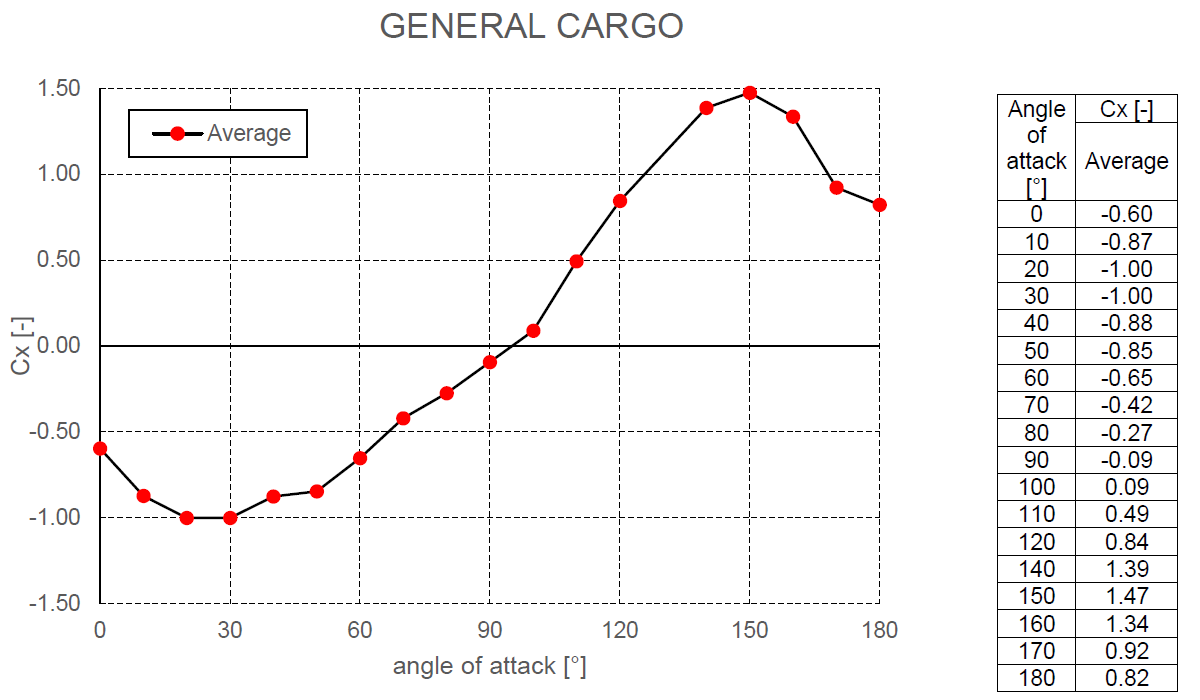
\includegraphics[width=0.9\linewidth]{wind cx.png}  
	\caption{Data sets of the wind resistance coefficient $C_{x}$ for general cargos}  
	\label{windCx}  
\end{figure}
\noindent For convenience, $C_{x}(130^{\circ})$ would be calculated, and $C_{x}$ would be extended to 360 degrees while each element in $C_{x_extended}$ be changed to its own opposite value. Then, based on Assumption (\ref{A10}), Eq.(\ref{wind1}) would be rewritten as:
\begin{equation}
    R_{wind}=\frac{1}{2} \rho_{A} C_{x_extended}\left(\psi_{\text {WR}}\right) A_{X V} V_{\text {WR}}^{2}-\frac{1}{2} \rho_{A} C_{x_extended}(0) A_{X V} V_{G}^{2}
    \label{wind2}
\end{equation}
where:
\begin{equation*}
    V_{\text {WR}}=\sqrt{V_{\text {WT}}^{2}+V_{\mathrm{G}}^{2}+2 V_{\text {WT}} V_{\mathrm{G}} \cos \left(\psi_{\text {WT}}-\psi\right)}
\end{equation*}
\begin{equation*}
    \begin{aligned}
        &\text{If:} \quad V_{\mathrm{G}}+V_{\mathrm{WT}} \cos \left(\psi_{\mathrm{WT}}-\psi\right) \geq 0\\
        &\quad \psi_{\mathrm{WR}}=\tan ^{-1} \frac{V_{\mathrm{WT}} \sin \left(\psi_{\mathrm{WT}}-\psi\right)}  {V_{\mathrm{G}}+V_{\mathrm{WT}} \cos \left(\psi_{\mathrm{WT}}-\psi\right)} \\
        &\quad \text{Range:} -90^{\circ} \sim 90^{\circ} \\
        &\text{If:} \quad V_{\mathrm{G}}+V_{\mathrm{WT}} \cos \left(\psi_{\mathrm{WT}}-\psi\right)<0\\
        &\quad \psi_{\mathrm{WR}}=\tan ^{-1} \frac{V_{\mathrm{WT}} \sin \left(\psi_{\mathrm{WT}}-\psi\right)}{V_{\mathrm{G}}+V_{\mathrm{WT}} \cos \left(\psi_{\mathrm{WT}}-\psi\right)}+180^{\circ} \\
        &\quad \text{Range:} -90^{\circ} \sim 90^{\circ} \quad \text{and} \quad 90^{\circ} \sim 270^{\circ} \\
        &\text{Then, if:} \quad \psi_{\mathrm{WR}} < 0\\
        &\quad \psi_{\mathrm{WR}}=\psi_{\mathrm{WR}}+360^{\circ}\\
        &\quad \text{Range:} 0^{\circ} \sim 90^{\circ} \quad \text{and} \quad 90^{\circ} \sim 270^{\circ} \quad \text{and} \quad 270^{\circ} \sim 360^{\circ}\\
    \end{aligned}
\end{equation*}
After getting $R_{wind}$, we could calculate cost caused by wind. The (part of) function for calculating cost caused by wind could be found in \autoref{calcostwind}.
\subsubsection{Cost caused by wave}
\label{Cost Wave}
Cost caused by wave is similar than that caused by wind, which needs to be separated as 4 parts. According to Eq.(\ref{STAwave}) and based on Assumption (\ref{A7}), this function could be found in \autoref{calcostwave}.
\subsubsection{Cost caused by the reaction between hull and calm water}
\label{Cost Hull}
According to Molland's work \cite{molland2011ship}, based on Assumption (\ref{A12}), coefficients $a \sim h$ would be shown as below:
\begin{table}[H]
    \begin{center}
        \caption{Coefficients of Hollenbach method}
        \label{HolCoeff}
        \resizebox{1\linewidth}{!}{
            \begin{tabular}{|c|c|c|c|c|c|c|c|c|c|}
                \hline
                a1       & a2       & a3       & a4                 & a5                & a6     & a7            & a8                     & a9                & a10                \\ \hline
                -0.3382  & 0.8086   & -6.0258  & -3.5632            & 9.4405            & 0.0146 & 0             & 0                      & 0                 & 0                  \\ \hline
                b11      & b12      & b13      & \multicolumn{2}{c|}{\multirow{8}{*}{}} & d1     & d2            & d3                     & \multicolumn{2}{c|}{\multirow{8}{*}{}} \\ \cline{1-3} \cline{6-8}
                -0.57424 & 13.3893  & 90.596   & \multicolumn{2}{c|}{}                  & 0.854  & -1.228        & 0.497                  & \multicolumn{2}{c|}{}                  \\ \cline{1-3} \cline{6-8}
                b21      & b22      & b23      & \multicolumn{2}{c|}{}                  & e1     & e2            & \multirow{2}{*}{}      & \multicolumn{2}{c|}{}                  \\ \cline{1-3} \cline{6-7}
                4.6614   & -39.721  & -351.483 & \multicolumn{2}{c|}{}                  & 2.1701 & -0.1602       &                        & \multicolumn{2}{c|}{}                  \\ \cline{1-3} \cline{6-8}
                b31      & b32      & b33      & \multicolumn{2}{c|}{}                  & f1     & f2            & f3                     & \multicolumn{2}{c|}{}                  \\ \cline{1-3} \cline{6-8}
                -1.14215 & -12.3296 & 459.254  & \multicolumn{2}{c|}{}                  & 0.17   & 0.2           & 0.6                    & \multicolumn{2}{c|}{}                  \\ \cline{1-3} \cline{6-8}
                g1       & g2       & g3       & \multicolumn{2}{c|}{}                  & h1     & \multicolumn{2}{c|}{\multirow{2}{*}{}} & \multicolumn{2}{c|}{}                  \\ \cline{1-3} \cline{6-6}
                0.642    & -0.635   & 0.15     & \multicolumn{2}{c|}{}                  & 1.204  & \multicolumn{2}{c|}{}                  & \multicolumn{2}{c|}{}                  \\ \hline
            \end{tabular}
        }
    \end{center}
\end{table}
\noindent In addition, a matlab scrip has been given in blackboard, which has been rewritten as a Python script (\autoref{oricalcosthull}).
\\Based on this script and according to Eq.(\ref{total resistance}) and Eq.(\ref{RHullEq}), the above script would be modified. The modified version could be found in \autoref{calcosthull}.
\subsection{Path finding}
\label{Pathfinding}
This part is discussed with Ziwen Wang (Student number:546844).
\\For better display, this work for path finding is modified based on an open source project written by Atsushi, which aims for a robot to plan a path rounding obstacles. 
\\In Atsushi's project, there are some obstacles and robot has its own radius. So, this robot could move in 8 different directions and find the shortest way to round these obstacles and arrive the goal point by Dijkstra algorithm. In this case, the cost between any two neighbour nodes is set to the same. Here is an example below (result of \autoref{Atsushi}):
\begin{figure}[H]
    \centering  
	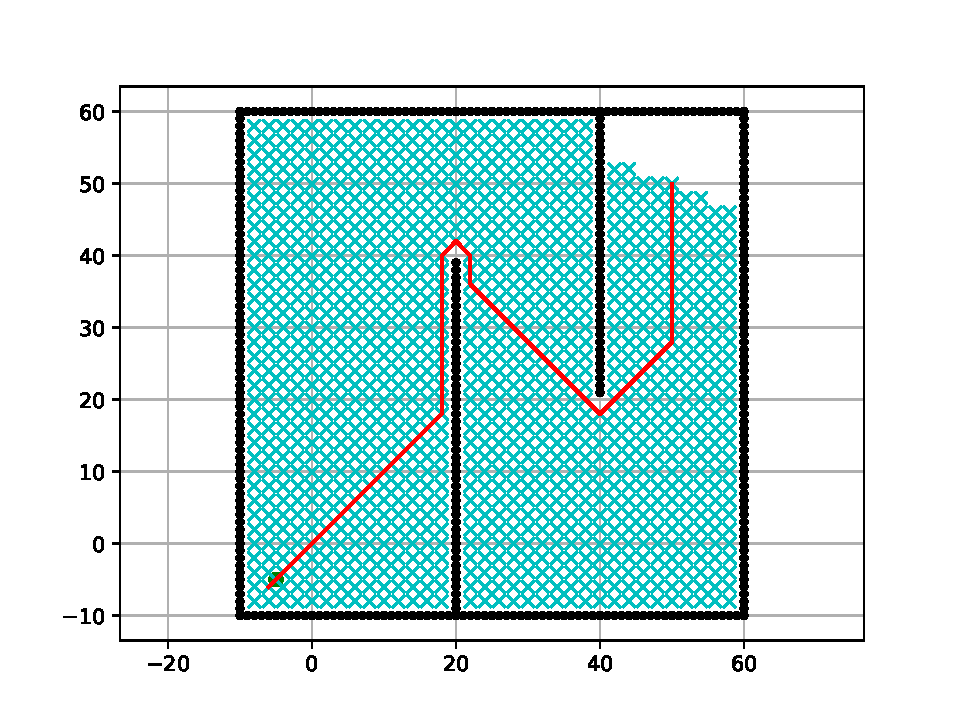
\includegraphics[width=0.9\linewidth]{OriginDijkstra.pdf}  
	\caption{Grid based Dijkstra planning (Atsushi's project)}
\end{figure}
\noindent However, some of these principles in Atsushi's project are against previous assumptions, in which case some modifications are necessary. 
\\Based on Assumption (\ref{A4}) and (\ref{A7}), the number of movement directions would be deleted to four. Owing to Assumption (\ref{A13}), all obstacles are removed. The robot radius, which could be considered as the beam of ship, would be discarded as well because of Assumption (\ref{A14}). This removal just eliminates the influence of beam on ship movement to ensure that this ship could move on all nodes in grid, even those nodes on the boundaries, but it does not mean that the effect of beam on resistance would be changed. In final, owing to the influence of ship heading angle, cost of movements between two nodes has an independent value for each direction. So, to find the path whose cost is minimum in a given velocity, the cost of each direction on every node would be replaced by calculated results in above sections.  After finding efficient path, the cost of this path could be given. According to Eq.(\ref{costfundt}), total cost of each path could be expressed as:
\begin{equation}
    C_{total}(V_{G,j})=\sum_{n=1}^N \Delta C_{n}(V_{G,j})
\end{equation}
\begin{itemize}
    \item $C_{total}(V_{G,j})$: Total cost of the voyage for the given velocity $V_{G,j}$
    \item $\Delta C_{n}$: Cost per section of this path, $\Delta C_{1}$ means the cost from the start point to the first driving point,  $\Delta C_{1}$ means the cost from the last point before the end to the goal point
\end{itemize}
The modified version could be found in \autoref{moddijk}.
\subsection{Velocity picking}
\label{Effective velocity}
The minimum velocity could be defind as:
\begin{equation}
    \begin{aligned}
        V_{min}&=\frac{l_{min}}{t}
        &=\frac{(|sx-gx|+|sy-gy|)*dist}{t}
    \end{aligned}
\end{equation}
\begin{itemize}
    \item $V_{min}$: Minimum velocity
    \item $l_{min}$: Length of shortest path
    \item $sx$: x position of the start point
    \item $gx$: x position of the goal point
    \item $sy$: y position of the start point
    \item $gy$: y position of the goal point
    \item $dist$: distance between two neighbour nodes
\end{itemize}
The maximum velocity could be defind as:
\begin{equation}
    \begin{aligned}
        V_{max}&=\frac{l_{max}}{t}
        &=\frac{(xcol \cdot yrow)*dist}{t}
    \end{aligned}
\end{equation}
\begin{itemize}
    \item $V_{max}$: Maximum velocity
    \item $l_{max}$: Length of longest path
    \item $xcol$: Number of columns in grid
    \item $yrow$: Number of rows in grid 
\end{itemize}
However, if each velocity would be calculated in program, it will cause computing time too long. So, setting a iteration limitation would be a good idea to improve efficiency.
\\After comparing total costs of efficient paths under different velocities, we could choose the optimal speed. Codes for this function could be found in \autoref{ChoOptVel}.